%%%%%%%%%%%%%%%%%%%%%%%%%%%%%%%%%%%%%%%%%
% Stylish Article
% LaTeX Template
% Version 2.1 (1/10/15)
%
% This template has been downloaded from:
% http://www.LaTeXTemplates.com
%
% Original author:
% Mathias Legrand (legrand.mathias@gmail.com) 
% With extensive modifications by:
% Vel (vel@latextemplates.com)
%
% License:
% CC BY-NC-SA 3.0 (http://creativecommons.org/licenses/by-nc-sa/3.0/)
%
%%%%%%%%%%%%%%%%%%%%%%%%%%%%%%%%%%%%%%%%%

%----------------------------------------------------------------------------------------
%	PACKAGES AND OTHER DOCUMENT CONFIGURATIONS
%----------------------------------------------------------------------------------------

\documentclass[fleqn,10pt]{SelfArx} % Document font size and equations flushed left

\usepackage[english]{babel} % Specify a different language here - english by default

\usepackage{listings}
\usepackage{lipsum} % Required to insert dummy text. To be removed otherwise

\lstset{
  basicstyle=\ttfamily,
  columns=fullflexible,
  frame=single,
  breaklines=true,
  postbreak=\mbox{\textcolor{red}{$\hookrightarrow$}\space},
}

%----------------------------------------------------------------------------------------
%	COLUMNS
%----------------------------------------------------------------------------------------

\setlength{\columnsep}{0.55cm} % Distance between the two columns of text
\setlength{\fboxrule}{0.75pt} % Width of the border around the abstract

%----------------------------------------------------------------------------------------
%	COLORS
%----------------------------------------------------------------------------------------

\definecolor{color1}{RGB}{0,0,90} % Color of the article title and sections
\definecolor{color2}{RGB}{0,20,20} % Color of the boxes behind the abstract and headings

%----------------------------------------------------------------------------------------
%	HYPERLINKS
%----------------------------------------------------------------------------------------

\usepackage{hyperref} % Required for hyperlinks
\hypersetup{hidelinks,colorlinks,breaklinks=true,urlcolor=color2,citecolor=color1,linkcolor=color1,bookmarksopen=false,pdftitle={Title},pdfauthor={Author}}

%----------------------------------------------------------------------------------------
%	ARTICLE INFORMATION
%----------------------------------------------------------------------------------------

\JournalInfo{Proyecto HPC} % Journal information
\Archive{EAFIT} % Additional notes (e.g. copyright, DOI, review/research article)

\PaperTitle{Proyecto HPC} % Article title

\Authors{Lope Carvajal\textsuperscript{1}, Samuel Sarabia\textsuperscript{2}} % Authors
\affiliation{\textsuperscript{1}\textit{Ingeniería de Sistemas, Universidad EAFIT, Medellin, Colombia, lcarva12@eafit.edu.co}} % Author affiliation
\affiliation{\textsuperscript{2}\textit{Ingeniería de Sistemas, Universidad EAFIT, Medellin, Colombia, ssarabia@eafit.edu.co}} % Author affiliation

\Keywords{Big Data, K-Means, Pyspark, Clusters, Spark, Pipeline, RDD, Dataframe, Python} % Keywords - if you don't want any simply remove all the text between the curly brackets
\newcommand{\keywordname}{Keywords} % Defines the keywords heading name

%----------------------------------------------------------------------------------------
%	ABSTRACT
%----------------------------------------------------------------------------------------

\Abstract{
En el presente artículo se explicará el funcionamiento y los procedimientos que realiza el algoritmo k-means. Además se abordará el tema de el análisis de eficiencia en la ejecución de este por medio de SPARK.
El análisis abarca una diversa comparación de resultados de tiempos de ejecución en diferentes circunstancias donde se ha probado el código realizado.
Además de esto, se documentará el código realizado para solucionar este análisis, dando a entender con mayor claridad la forma en que se está ejecutando y estamos llegando a dichos resultados.
Para la implementación del algoritmo utilizamos Pyspark, haciendo énfasis en la librería MLlib para el uso de la implementación de K-Means.
Por otro lado, se realizará una comparación de eficiencia entre una implementación previamente realizada de HPC y esta, enfocada a Big Data.
}

%----------------------------------------------------------------------------------------

\begin{document}

\flushbottom % Makes all text pages the same height

\maketitle % Print the title and abstract box

\tableofcontents % Print the contents section

\thispagestyle{empty} % Removes page numbering from the first page

%----------------------------------------------------------------------------------------
%	ARTICLE CONTENTS
%----------------------------------------------------------------------------------------

\section*{Introducción} % The \section*{} command stops section numbering

\addcontentsline{toc}{section}{Introducción} % Adds this section to the table of contents

El proyecto presentó un gran reto para nosotros, y este fue el aprendizaje de la herramienta Spark, junto con implementaciones que se encuentran implicitamente implicadas con el uso de la misma, tal es el caso de HDFS por dar un ejemplo.
En comparación al programa previamente realizado para el módulo de HPC, el desarrollo se hizo más corto en el proceso de codificación, pues gracias al uso de la librería MLlib no fue necesario realizar el algoritmo de K-Means explicitamente. Pero por otro lado la comprensión de la librería y como se debíá ejecutar el código se hizo similarmente dificultoso.

INCLUIR RESULTADOS DE LAS PRUEBAS

%------------------------------------------------

\section{Marco Teorico}

\subsection{Definición del Problema}

Para abarcar el análisis del presente documento, es importante  dar una descripción detallada del problema que vamos a solucionar. Como se había mencionado anteriormente, se aborda el problema de clasificación de textos por medio de su similaridad utilizando el algoritmo de K-means, con encontrando el cálculo de las distancias entre documentos por medio de la aplicación de la medida numérica Tf-idf(Term frequency -Inverse Document frequency)

\subsection{Análisis de Texto}

Para poder comenzar a comparar para encontrar qué tan similares son dos documentos, debemos primero convertirlos en alguna estructura matemática de datos. 
Primero es necesario eliminar las palabras conectoras y artículos del lenguaje en el que se encuentren los textos. El algoritmo sólo eliminará las palabras conectoras de un lenguaje. La librería nos brinda una lista con estas palabras que después eliminamos.
A partir de la lista con los elementos relevantes se aplica el algoritmo de Tf-idf, donde se obtiene el número de veces que un término aparece en un documento y la relevancia del mismo en la totalidad de documentos que se están evaluando.

\begin{equation}
IDF(t,D)=\log \frac{|x| + 1}{DF(t,D)+1}
\label{eq:refname2}
\end{equation}

\subsection{K-means}
K-means es uno de los algoritmos no supervisados más simples para resolver el problema de agrupamiento. El proceso sigue una forma simple de clasificar un dataset en un número predeterminado de clusters. La idea en resumen es definir k centros, uno por cada cluster. Estos centros, en algunos casos, son asignados en primera instancia de forma aleatoria, aunque existen diversas implementaciones de este paso para hacer el algoritmo más efectivo, ya que diferentes ubicaciones de los centros conducen a diferentes resultados.
El siguiente paso es tomar cada punto del dataset otorgado y relacionarlo con el centro más cercano, cuando no quedan más puntos, el primer paso es completado y un agrupamiento simple es realizado.
En este punto se deben recalcular k nuevos centros ubicados en el promedio de la agrupación realizada en la primera iteración. Después de tener estos k nuevos centros, una nueva agrupación debe ser realizada entre éstos y el dataset inicial.
De este modo se crea un ciclo que termina cuando los centros nuevos son equivalentes a los previamente calculados y arroja el resultado.

\begin{equation}
MIN \sum_{j=1}^{k} \sum_{i=1}^{n} \lvert \lvert x-\mu_j \lvert \lvert^{2}  
\label{eq:refname2}
\end{equation}
%------------------------------------------------

\section{Análisis y diseño mediante analítica de datos}

\begin{figure}[ht]\centering
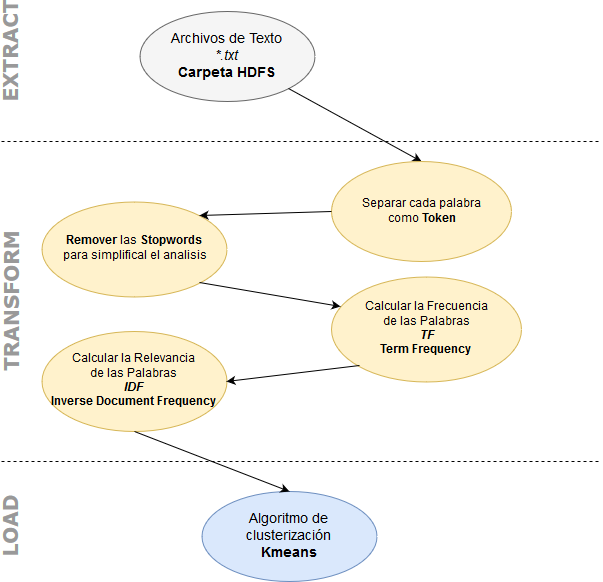
\includegraphics[width=85mm,]{ETL}
\caption{Flujo ETL}
\label{fig:tabla1}
\end{figure}
\subsection{Extract}
\begin{itemize}
\item Para la extracción de datos se accede a un directorio ubicado en el HDFS de la máqina, de allí se extraen todos los archivos de texto por medio del método wholeTextFiles() contenido en Pyspark, que devuelve un RDD que contiene estos datos.
\end{itemize}
\subsection{Transform}

\begin{itemize}
  \item Se separan las palabras como Tokens, y se guardan como una lista con uno en cada posición.
  \item Se realiza un proceso de remoción de stopwords para simplificar el análisis y se ignoren las palabras que no son útiles para la comparación.
  \item Se calcula la frecuencia de las palabras en cada documento y la relevancia de las mismas dentro de todos los documentos.
\end{itemize}





\subsection{Load}
\begin{itemize}
\item Se pasan los datos previamente procesados al algoritmo de clusterización para que termine la ejecución.
\end{itemize}





\section{Implementación}
Hay tres lenguajes compatibles con Spark, estos son:
\begin{itemize}
  \item Scala
  \item Java
  \item Python
\end{itemize}
Para nuestra implementación decidimos utilizar Python, más específicamente Pyspark.

En primer lugar, se crea un RDD con todos los archivos de texto de una carpeta específica.

\begin{lstlisting}[language=Python]
files = sc.wholeTextFiles("hdfs:///user/lcarva12/pruebaKmeans")
\end{lstlisting}

Posteriormente se crea un esquema para convertirlo en un dataframe que contiene el path y el texto del archivo.

\begin{lstlisting}[language=Python]
schema =  StructType([StructField ("path" , StringType(), True) , 
StructField("text" , StringType(), True)]) 
df = spark.createDataFrame(files,schema)
\end{lstlisting}

En base al texto de cada uno de los archivos se crea una lista con todas las palabras separadas.
	
\begin{lstlisting}[language=Python]
tokenizer = Tokenizer(inputCol="text", outputCol="tokens")
\end{lstlisting}	

A esta lista se le extraen las palabras que no son necesarias, como artículos y conectores.

\begin{lstlisting}[language=Python]
remover = StopWordsRemover(inputCol="tokens", outputCol="stopWordsRemovedTokens")
\end{lstlisting}

Después de esto se realiza el proceso previamente mencionado para calcular el Tf-idf

\begin{lstlisting}[language=Python]
hashingTF = HashingTF(inputCol="stopWordsRemovedTokens", outputCol="rawFeatures", numFeatures=2000)
idf = IDF(inputCol="rawFeatures", outputCol="features", minDocFreq=5)

\end{lstlisting}

En base a esto se ejecuta el algoritmo de K-Means.

\begin{lstlisting}[language=Python]
kmeans = KMeans(k=5)
pipeline = Pipeline(stages=[tokenizer, remover, hashingTF, idf, kmeans])
model = pipeline.fit(df)
results = model.transform(df)
\end{lstlisting}

Todo este proceso se realiza mediante la definición y posterior ejecución de un pipeline donde se encuentran todas las operaciones previamente mencionadas.

\begin{figure}[ht]\centering
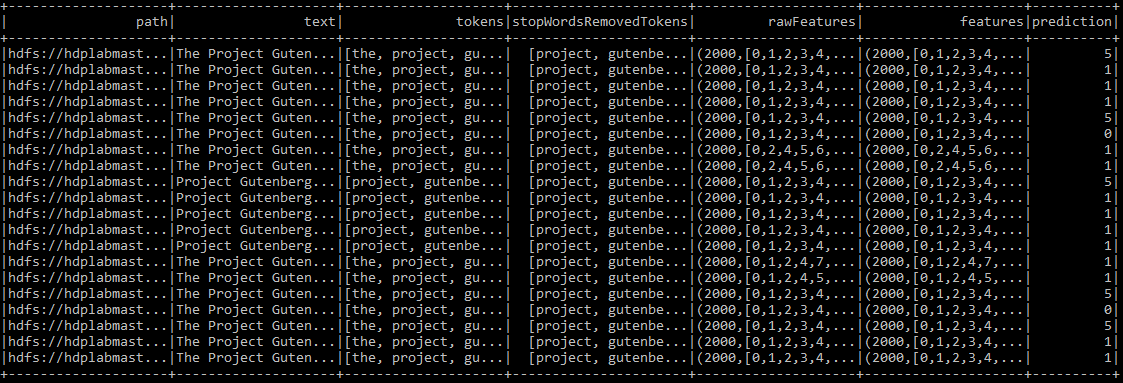
\includegraphics[width=80mm,]{Resultado}
\caption{Resultados ejecución con 500 archivos}
\label{fig:tabla1}
\end{figure}

%------------------------------------------------
\section{Pruebas}
%------------------------------------------------
Se realizaron diversas pruebas para comparar el rendimiento y la diferencia entre la implementación realizada para el módulo de HPC y el de Big Data. 
Para estas pruebas se utilizaron diferentes cantidades de documentos del dataset proveído por Gutenberg(Incluyendo una prueba donde se realiza clustering de todos los documentos) para analizar como se desenvolvía el algoritmo en diferentes escenarios.
La realización del primer test se justificó bajo la búsqueda de una comparación con la ejecución paralela de K-Means relaizada en el módulo pasado. Para estas pruebas se utilizaron tres escenarios:
\begin{itemize}
  \item 500 documentos del dataset Gutenberg clasificados en 4 clusters.
  \item 1000 documentos del dataset Gutenberg clasificados en 6 clusters.
  \item Dataset Gutenberg completo clasificados en 8 clusters.
\end{itemize}

\begin{figure}[ht]\centering
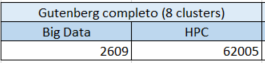
\includegraphics[width=50mm,]{hvb1}
\caption{Resultados ejecución Gutenberg completo}
\label{fig:tabla1}
\end{figure}

\begin{figure}[ht]\centering
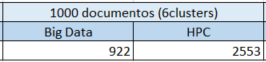
\includegraphics[width=50mm,]{hvb2}
\caption{Resultados ejecución 1000 documentos}
\label{fig:tabla1}
\end{figure}

\begin{figure}[ht]\centering
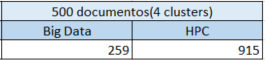
\includegraphics[width=50mm,]{hvb3}
\caption{Resultados ejecución 500 documentos}
\label{fig:tabla1}
\end{figure}

Con estos resultados se puede apreciar que la implementación de Big Data es más eficiente para realizar el clustering de documentos por medio del algoritmo de KMeans. La diferencia de tiempo de ejecución es por poco abismal cuando se trata de una cantidad relativamente grande de archivos, como son los aproximadamente tres mil archivos de texto contenidos en la biblioteca de Gutenberg.

\begin{figure}[ht]\centering
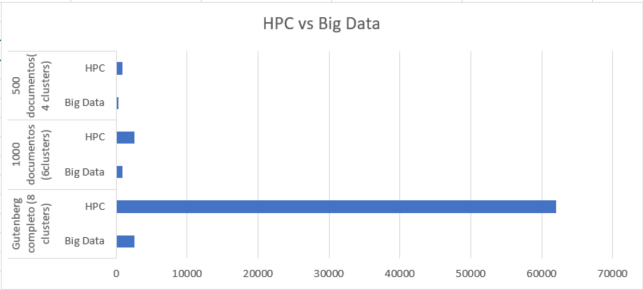
\includegraphics[width=85mm,]{chart1}
\caption{Comparación de tiempos de ejecución en segundos}
\label{fig:tabla1}
\end{figure}

%------------------------------------------------
\section{Conclusión}
%------------------------------------------------

Spark provee grandes ventajas para la resolución de problemas de Big Data como el tratado en este documento, siendo este la clasificación de documentos por medio del algoritmo de K-Means.

\noindent Esta implementación fue sustancialmente más sencilla que la del módulo pasado, pues las herramientas disponibles para atacar el problema por medio de Pyspark facilitan el proceso y hacen que este sea mucho más corto.

\noindent Además de esto, se obtiene un código más legible y entendible, ya que muchas partes de la secuencia son casi legibles en lenguaje natural.

\noindent La implementación actual superó con creces la realizada para el módulo de HPC en términos de rendimiento, pues gracias a la ejecución de pruebas se comprobó que la diferencia es muy singificativa, alcanzando que en una gran cantidad de archivos a procesar se tardara hasta 27 veces menos la clasificación de los mismos.

\noindent Una causa de esta diferencia en tiempo de ejecución se debe a nuestra incapacidad de paralelizar la sección del algoritmo de K-Means en el proyecto pasado, donde se distribuyó únicamente la sección donde se procesaban los documentos para entregarselos a dicho algoritmo.

\noindent Esta dificultad se tuvo por la forma en que planteamos el problema, ya que no hicimos una división correcta del mismo para que fuera paralelizado más facilmente.



%------------------------------------------------
\phantomsection
\section*{Acknowledgments} % The \section*{} command stops section numbering
Utilizamos el git\cite{git} como base para la implementación de nuestra solución.

\addcontentsline{toc}{section}{Acknowledgments} % Adds this section to the table of contents



%----------------------------------------------------------------------------------------
%	REFERENCE LIST
%----------------------------------------------------------------------------------------
\phantomsection
\bibliographystyle{unsrt}

\begin{thebibliography}{9}
\bibitem{Huang} 
Anna Huang
\textit{Similarity measures for text document clustering.} 
Proceedings of the Sixth New Zealand, April):49–56, 2008. 

 
\bibitem{Info Retrieval} 
Christopher D. Manning, Prabhakar Raghavan, and Hinrich Schütze.
\textit{Introduction to Information Retrieval}.  
Cambridge University Press, 2008
 
\bibitem{git} 
MLlib,
$https://spark.apache.org/mllib/$

\bibitem{nltk}
Pyspark,
$https://pypi.python.org/pypi/pyspark$ 

\end{thebibliography}

%----------------------------------------------------------------------------------------

\end{document}